\begin{englishtitle} % Настраивает LaTeX на использование английского языка
% Этот титульный лист верстается аналогично.
\title{Asymptotic solutions of the nonlocal kinetic equation of ionization of an active medium with cubic nonlinearity}
% First author
\author{S.A. Siniukov
}
\institute{TSU, Tomsk, Russia\\
  \email{ssaykmh@yandex.ru}
  }

% etc

\maketitle

\begin{abstract}
An original semiclassical approach is used to solve a two-dimensional kinetic equation with nonlocal cubic nonlinearity, which is a model of ionization of an active medium. The considered asymptotic solutions are constructed analytically in the class of trajectory concentrated functions in the weak diffusion approximation. Analytical and numerical methods were used to study the dependence of the discrepancy of the asymptotic solution on time and on the asymptotic small parameter. The consistency of asymptotic and numerical solutions in the selected range of model parameters is shown.

\keywords{active media, nonlocal kinetic equation, asymptotic solutions, semiclassical asymptotics, WKB-Maslov method, discrepancy} % в конце списка точка не ставится
\end{abstract}
\end{englishtitle}

\iffalse
%%%%%%%%%%%%%%%%%%%%%%%%%%%%%%%%%%%%%%%%%%%%%%%%%%%%%%%%%%%%%%%%%%%%%%%%
%
%  This is the template file for the 6th International conference
%  NONLINEAR ANALYSIS AND EXTREMAL PROBLEMS
%  June 25-30, 2018
%  Irkutsk, Russia
%
%%%%%%%%%%%%%%%%%%%%%%%%%%%%%%%%%%%%%%%%%%%%%%%%%%%%%%%%%%%%%%%%%%%%%%%%



\documentclass[12pt]{llncs}

% При использовании pdfLaTeX добавляется стандартный набор русификации babel.
% Если верстка производится в LuaLaTeX, то следующие три строки надо
% закомментировать, русификация будет произведена в корректирующем стиле автоматом.
\usepackage{iftex}

\ifPDFTeX
\usepackage[T2A]{fontenc}
\usepackage[utf8]{inputenc} % Кодировка utf-8, cp1251 и т.д.
\usepackage[english,russian]{babel}
\fi

% Для верстки в LuaLaTeX текст готовится строго в utf-8!

% В операционной системе Windows для редактирования в кодировке utf-8
% можно использовать программы notepad++ https://notepad-plus-plus.org/,
% techniccenter http://www.texniccenter.org/,
% SciTE (самая маленькая по объему программа) http://www.scintilla.org/SciTEDownload.html
% Подойдет также и встроенный в свежий дистрибутив MiKTeX редактор
% TeXworks.

% Добавляется корректирующий стилевой файл строго после babel, если он был включен.
% В параметре необходимо указать russian, что установит не совсем стандартные названия
% разделов текста, настроит переносы для русского языка как основного и т.п.

\usepackage{todonotes} % Этот пакет нужен для верстки данного шаблона, его
                       % надо убрать из вашей статьи.

\usepackage[russian]{nla}


\begin{document}
\fi

\title{Асимптотические решения нелокального кинетического уравнения ионизации активной среды с кубичной нелинейностью}
% Первый автор
\author{С.~А.~Синюков
 % \and
% Второй автор
 % А.~Е.~Кулагин\inst{2}
 % \and
% Третий автор
 % А.~В.~Шаповалов\inst{1}
}

% Аффилиации пишутся в следующей форме, соединяя каждый институт при помощи \and.
\institute{НИ ТГУ, Томск, Россия \\
  \email{ssaykmh@yandex.ru}
 % \and   % Разделяет институты и присваивает им номера по порядку.
%НИ ТПУ, Томск, Россия\\
 % \email{aek8@tpu.ru}
% \and Другие авторы...
}

\maketitle

\begin{abstract}
Применяется оригинальный квазиклассический подход для решения двумерного кинетического уравнения с нелокальной кубичной нелинейностью, являющегося моделью ионизации активной среды. Рассматриваемые асимптотические решения построены аналитически в классе траекторно-сосредоточенных функций в приближении слабой диффузии. Аналитическими и численными методами проведено исследование зависимости невязки асимптотического решения от времени и от асимптотического малого параметра. В выбранной области значений параметров модели показана согласованность асимптотических и численных решений.

\keywords{активная среда, нелокальное кинетическое уравнение, асимптотические решения, квазиклассические асимптотики, метод ВКБ–Маслова, невязка} % в конце списка точка не ставится
\end{abstract}

%\section{Основные результаты} % не обязательное поле

Метод квазиклассически сосредоточенных состояний, основанный на теории ростка Маслова является мощным инструментом построения асимптотических решений нелокальных нелинейных уравнений.

В данной работе исследуются свойства асимптотических решений нелокальной модели ионизации активной среды на парах металлов (АСПМ) \cite{Little}, построенных методом квазиклассически сосредоточенных состояний \cite{ShKulSin}. Уравнение АСПМ описывает двумерное распределение концентрации ионов в активной среде в поперечном сечении газоразрядной трубки (ГРТ) в предположении его однородности вдоль оси ГРТ \cite{CarBrPip}.  Проведен сравнительный анализ асимптотических и численных решений уравнения АСПМ при одинаковых начальном условии и параметрах модели. Сравнение численных и асимптотических решений (рис.\ref{fig1}) показало, что при уменьшении асимптотического параметра диффузии асимптотические решения приближаются к численным, что говорит о справедливости асимптотического метода, примененного в  \cite{ShKulSin} в выбранной области значений параметров модели. Исследование невязки продемонстрировало, что в некоторой области достаточно малых значений параметра   асимптотическое решение имеет точность $O(D^{3/2})$, что согласуется с оценками асимптотических решений.



% Рисунки и таблицы оформляются по стандарту класса article. Например,

\begin{figure}[htb]
  \centering
  % Поддерживаются два формата:
  %\includegraphics[width=0.7\linewidth]{figure.pdf} % Растровый формат
  %\includegraphics[width=0.7\linewidth]{figure.png} % Векторный и растровый формат
  %

  \begin{center}
    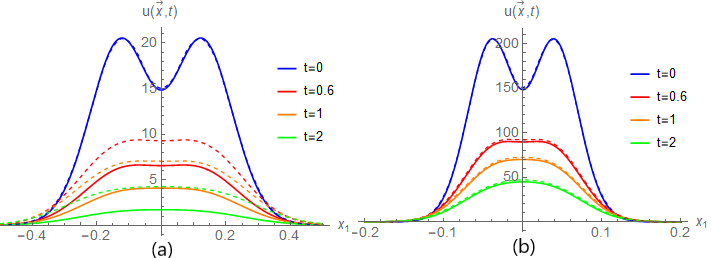
\includegraphics[width=0.8\linewidth]{D01Resh.png}
  \end{center}
  \caption{Асимптотические (сплошные линии) и численные (пунктирные линии) решения уравнения АСПМ при (a) - $D=0.01$, (b) - $D=0.001$ и $\Vec{x}=(x_1,0)$.}\label{fig1}
\end{figure}


Применение квазиклассического метода для получения асимптотических решений диссипативных задач дает ряд преимуществ. Квазиклассические асимптотики имеют растущую во времени ошибку \cite{HagJo}. Однако для открытых систем с затухающими процессами ошибка будет ограничена сверху, так как невязка убывает, начиная с некоторого момента времени.

% В конце текста можно выразить благодарности, если этого не было
% сделано в ссылке с заголовка статьи, например,
%Работа выполнена при поддержке РФФИ (РНФ, другие фонды), проект \textnumero~00-00-00000.
%



\begin{thebibliography}{9} % или {99}, если ссылок больше десяти.
\bibitem{Little} Little C.E. Metal vapor lasers: Physics, Engineering and Applications.  Chichester, UK: John Willey and Sons Ltd., 1998 . P. 620.
\bibitem{ShKulSin} Shapovalov A.V. Kulagin A.E. Siniukov S.A. Family of asymptotic solutions to the two-dimensional kinetic equation with a nonlocal cubic nonlinearity//Symmetry, v. 14, № 6, 2022. P. 577.
\bibitem{CarBrPip} Carman R.J., Brown D.J.W., A. Piper J.A. A self-consistent model for the discharge kinetics in a high-repetition-rate copper-vapor laser // IEEE Journal of Quantum Electronics, v. 30, № 8. 1994, P. 1876--1895.
\bibitem{HagJo} Hagedorn G., Joye A. Semiclassical dynamics with exponentially small error estimates//Comm. Math.  Phys, v. 207, 1999. P. 439--465.
\end{thebibliography}

% После библиографического списка в русскоязычных статьях необходимо оформить
% англоязычный заголовок.




%\end{document}
